\documentclass[convert]{standalone}

\usepackage{tikz}
\usetikzlibrary{calc}

\begin{document}
\begin{tabular}{cc}
  Before Collision & After Collision \\
  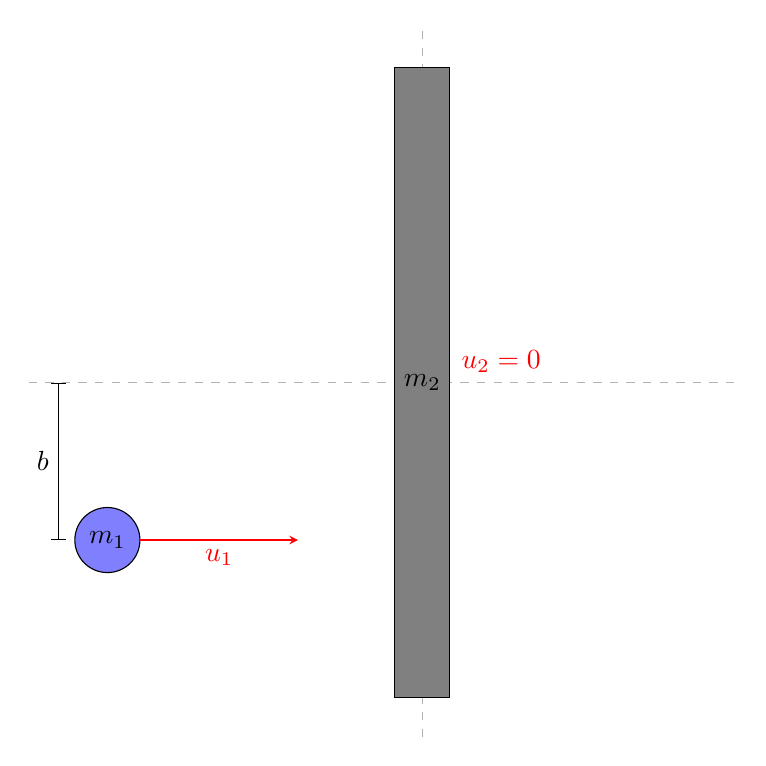
\begin{tikzpicture}[>=stealth]
    \draw[dashed,black!30!white] (-5,0) -- (4,0);
    \draw[dashed,black!30!white] (0,-4.5) -- (0,4.5);
    \node (stick) at (0,0) [rectangle,draw,fill=black!50!white,minimum height=8cm]{$m_2$};
    \node (puck) at (-4,-2) [circle,draw,fill=blue!50!white]{$m_1$};
    \draw [->,red] (puck.east) -- +(2,0) node[midway,below]{$u_1$};
    \node at ($(stick)+(1,0)$) [red,above]{$u_2=0$};
    \draw [|-|] ($(puck.west)+(-0.2,0)$) -- +(0,2) node[midway,left]{$b$};
  \end{tikzpicture}
    &
     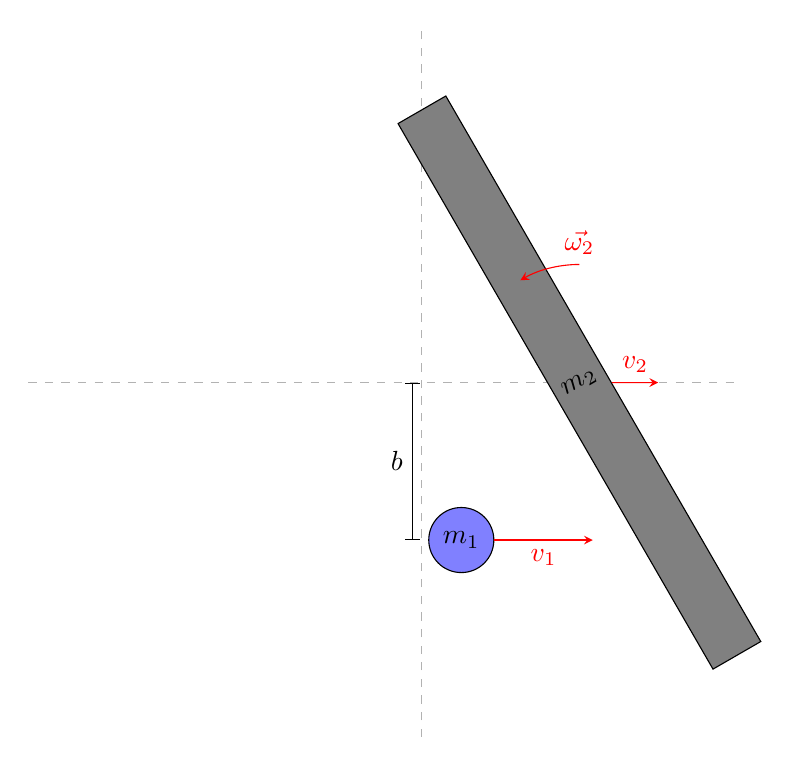
\begin{tikzpicture}[>=stealth]
       \draw[dashed,black!30!white] (-5,0) -- (4,0);
       \draw[dashed,black!30!white] (0,-4.5) -- (0,4.5);
       \node (stick) at (2,0) [rectangle,draw,fill=black!50!white,
                               minimum height=8cm,rotate=30]{$m_2$};
       \node (puck) at (0.5,-2) [circle,draw,fill=blue!50!white]{$m_1$};
       \draw [->,red] (puck.east) -- +(1.25,0) node[midway,below]{$v_1$};
       \draw [|-|] ($(puck.west)+(-0.2,0)$) -- +(0,2) node[midway,left]{$b$};
       \draw [->,red] (stick) -- +(1,0) node[midway,above]{$v_2$};
       \draw[->,red] ($(stick)+(0,1.5)$) node[above]{$\vec{\omega_2}$}
                     arc [start angle=90, end angle=120, radius=1.5cm];
     \end{tikzpicture}
 \\
\end{tabular}
\end{document}